\documentclass[tikz, border=4pt]{standalone}
\usepackage{tikz}
\usepackage{chemfig}
\begin{document}
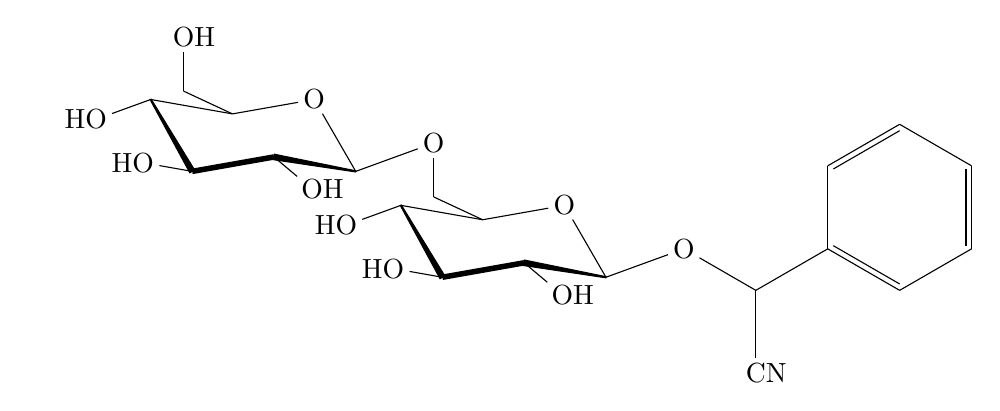
\begin{tikzpicture}[x=1cm, y=1cm]
  \node[anchor=north west, inner sep=0pt] at (0,0) {%
  \setchemfig{cram width=2pt}
  \definesubmol{c1}{-[:200]-[:120]O-[:190]}
  \definesubmol{c2}{-[:170](-[:200,0.7]HO)<[:300](-[:170,0.6]HO)
  -[:10,,,,line width=2pt](-[:-40,0.6]OH)>[:-10]}
  \definesubmol{csub}{-[:155,0.65]-[:90,0.65]}
  \chemfig{O(!{c1}(!{csub}O(!{c1}(!{csub}OH)!{c2}))!{c2})-[:-30](-[:-90]CN)-[:30]*6(=-=-=-)}%
  };
\end{tikzpicture}
\end{document}
